\documentclass[../../main.tex]{subfiles}
\begin{document}

{\bf [解]}

\begin{figure}[htb]
\begin{center}
\begin{tikzpicture}[scale=1.8, >=stealth]

  % --- 1. パラメータ設定 (例: theta = 70度, alpha = 215度) ---
  % 条件: 0 <= theta <= 180度, 180度 <= alpha <= theta + 180度
  \def\thetaVal{70}
  \def\alphaVal{215}

  % 原点 P
  \coordinate (P) at (0, 0);

  % 各円の中心 (原点からの距離 1)
  \coordinate (OA) at (1, 0);
  \coordinate (OB) at ({cos(\thetaVal)}, {sin(\thetaVal)});
  \coordinate (OC) at ({cos(\alphaVal)}, {sin(\alphaVal)});

  % --- 2. 中心の軌跡（単位円: 破線） ---
  \draw[dashed, gray!70] (P) circle (1.0);
  % \node[gray!80!black, font=\scriptsize, above right] at (0.7, 0.7) {中心の軌跡};

  % --- 3. 座標軸 ---
  \draw[->, thick, gray!80] (-2.2, 0) -- (2.3, 0) node[right, black] {$x$};
  \draw[->, thick, gray!80] (0, -2.1) -- (0, 2.1) node[above, black] {$y$};

  % --- 4. 3つの単位円板の描画 (半径 1) ---
  % 円 A (中心 OA)
  \draw[thick, blue!80!black] (OA) circle (1.0);
  \node[blue!80!black, font=\small, right] at (2.0, 0) {$A$};

  % 円 B (中心 OB)
  \draw[thick, red!80!black] (OB) circle (1.0);
  \node[red!80!black, font=\small, above] at ($({2*cos(\thetaVal)}, {2*sin(\thetaVal)})$) {$B$};

  % 円 C (中心 OC)
  \draw[thick, green!60!black] (OC) circle (1.0);
  \node[green!60!black, font=\small, below left] at ($({2*cos(\alphaVal)}, {2*sin(\alphaVal)})$) {$C$};

  % --- 5. 中心への動径（破線） ---
  \draw[thick, dashed, blue!80!black] (P) -- (OA);
  \draw[thick, dashed, red!80!black] (P) -- (OB);
  \draw[thick, dashed, green!60!black] (P) -- (OC);

  % --- 6. 偏角 theta, alpha の表示 ---
  % 偏角 theta
  \draw[->, thin, red!80!black] (0.45, 0) arc (0:\thetaVal:0.45);
  \node[red!80!black, font=\scriptsize] at ({\thetaVal/2}:0.6) {$\theta$};

  % 偏角 alpha
  \draw[->, thin, green!60!black] (0.32, 0) arc (0:\alphaVal:0.32);
  \node[green!60!black, font=\scriptsize] at ({\alphaVal/2 + 10}:0.45) {$\alpha$};

  % --- 7. 各点のプロットとラベル ---
  \fill[black] (P) circle (1.5pt) node[below left, font=\small] {$P$};

  \fill[blue!80!black] (OA) circle (1.5pt) node[below right, font=\small] {$O_A(1,0)$};
  \fill[red!80!black] (OB) circle (1.5pt) node[above, font=\small] {$O_B$};
  \fill[green!60!black] (OC) circle (1.5pt) node[below left, font=\small] {$O_C$};

\end{tikzpicture}
\end{center}
\caption{原点 $P$ を通る3つの単位円板 $A, B, C$ の配置（中心角 $\theta, \alpha$）}
\end{figure}

点$P$を原点$P(0,0)$とする．
3個の円板を$A,B,C$として回転して$A$の中心$O_A=(1,0)$に固定してよい．方程式は
\begin{align}
 A: \left(x-1\right)^2 + y^2 = 1 \label{eq:1}
\end{align}
となる．
$B,C$の中心$O_B,O_C$は単位円上にあるので偏角を$\theta,\alpha$とおく．
対称性から$B$は上半面にあるとしても一般性を失わないから
\begin{align}
 O_B=(\cos\theta,\sin\theta)\ (0\le\theta\le\pi) \label{eq:2}
\end{align}
とする．
最後の$O_C$は$O_B$よりも偏角が大きいとして一般性を失わないから
\begin{align}
  O_C=(\cos\alpha,\sin\alpha)\ (\theta\le\alpha\le2\pi) \label{eq:3}
\end{align}
とおく．
条件(b)を満たすような$\alpha$の範囲について考えよう．
まず$\theta \neq \pi$の時は$O_A$と$O_B$は$P$以外にも上半面に共有点を持つ．従ってこの領域で$O_C$が$O_A$と共有点を持ってはいけないから円の中心$O_C$が下半面になくてはならず，
\begin{align}
 \pi \le \alpha
\end{align}
である．
この時$\alpha \neq \pi$なら$O_A$と$O_C$は必ず下半面で$P$以外の共有点を持つから$O_C$が$O_B$と下半面で共有点を持ってはならず，$O_B$の原点対称な点（偏角$\pi+\theta$）よりも$O_C$の偏角が小さくないといけない：
\begin{align}
 \alpha \le \pi + \theta
\end{align}
従って条件(b)を満たす$O_C$の条件は
\begin{align}
\pi\le\alpha\le\theta+\pi\tag{①} \label{eq:4}
\end{align}
である．この時$P$以外では最大二つの円盤しか共通部分を持たない．

\begin{figure}[htb]
\begin{center}
\begin{tikzpicture}[scale=1.5, >=stealth]

  % ========================================================
  % 1. 左図: alpha < pi の場合 (例: theta = 120度, alpha = 60度)
  % ========================================================
  \begin{scope}[shift={(0, 0)}]
    \node[above, font=\bfseries] at (0.5, 2.3) {$\alpha < \pi$};

    \def\tL{120}
    \def\aL{60}

    \coordinate (P) at (0, 0);
    \coordinate (OA) at (1, 0);
    \coordinate (OB) at ({cos(\tL)}, {sin(\tL)});
    \coordinate (OC) at ({cos(\aL)}, {sin(\aL)});

    % 3円の三重重複部分 (NG領域) のハッチング
    \begin{scope}
      \clip (OA) circle (1.0);
      \clip (OB) circle (1.0);
      \fill[pattern=north east lines, pattern color=red!80!black] (OC) circle (1.0);
    \end{scope}

    % 座標軸
    \draw[->, thick, gray!80] (-1.8, 0) -- (2.3, 0) node[right, black] {$x$};
    \draw[->, thick, gray!80] (0, -1.6) -- (0, 2.3) node[above, black] {$y$};
    \node[below left, font=\scriptsize] at (P) {$P(0,0)$};

    % 中心の軌跡（単位円）
    \draw[dashed, gray!50] (P) circle (1.0);

    % 3つの円
    \draw[thick, blue!80!black] (OA) circle (1.0);
    \draw[thick, red!80!black]  (OB) circle (1.0);
    \draw[thick, green!60!black] (OC) circle (1.0);

    % 中心の動径
    \draw[dashed, blue!80!black] (P) -- (OA);
    \draw[dashed, red!80!black]  (P) -- (OB);
    \draw[dashed, green!60!black] (P) -- (OC);

    % 偏角の表示
    \draw[->, thin, green!60!black] (0.35, 0) arc (0:\aL:0.35);
    \node[green!60!black, font=\scriptsize] at (30:0.48) {$\alpha$};

    \draw[->, thin, red!80!black] (0.55, 0) arc (0:\tL:0.55);
    \node[red!80!black, font=\scriptsize] at (95:0.7) {$\theta$};

    % 各中心のプロット
    \fill[blue!80!black] (OA) circle (1.2pt) node[below right, font=\scriptsize] {$O_A$};
    \fill[red!80!black]  (OB) circle (1.2pt) node[above left, font=\scriptsize] {$O_B$};
    \fill[green!60!black] (OC) circle (1.2pt) node[above right, font=\scriptsize] {$O_C$};
    \fill[black] (P) circle (1.2pt);

    % 注記
    \node[red!80!black, font=\scriptsize, align=center] at (0.35, 0.95) {3円の重複\\(共有点あり)};
  \end{scope}

  % ========================================================
  % 2. 右図: alpha > theta + pi の場合 (例: theta = 50度, alpha = 270度 > 230度)
  % ========================================================
  \begin{scope}[shift={(4.8, 0)}]
    \node[above, font=\bfseries] at (0.5, 2.3) {$\alpha > \theta + \pi$};

    \def\tR{50}
    \def\aR{270}

    \coordinate (PR) at (0, 0);
    \coordinate (OAR) at (1, 0);
    \coordinate (OBR) at ({cos(\tR)}, {sin(\tR)});
    \coordinate (OCR) at ({cos(\aR)}, {sin(\aR)});

    % 3円の三重重複部分 (NG領域) のハッチング
    \begin{scope}
      \clip (OAR) circle (1.0);
      \clip (OBR) circle (1.0);
      \fill[pattern=north east lines, pattern color=red!80!black] (OCR) circle (1.0);
    \end{scope}

    % 座標軸
    \draw[->, thick, gray!80] (-1.8, 0) -- (2.3, 0) node[right, black] {$x$};
    \draw[->, thick, gray!80] (0, -2.1) -- (0, 2.1) node[above, black] {$y$};
    \node[above left, font=\scriptsize] at (PR) {$P(0,0)$};

    % 中心の軌跡（単位円）
    \draw[dashed, gray!50] (PR) circle (1.0);

    % 限界線 theta + pi (破線)
    \draw[dashed, purple!80!black, thick] (PR) -- ({cos(\tR+180)}, {sin(\tR+180)})
      node[below left, font=\scriptsize] {$\theta+\pi$};

    % 3つの円
    \draw[thick, blue!80!black] (OAR) circle (1.0);
    \draw[thick, red!80!black]  (OBR) circle (1.0);
    \draw[thick, green!60!black] (OCR) circle (1.0);

    % 中心の動径
    \draw[dashed, blue!80!black] (PR) -- (OAR);
    \draw[dashed, red!80!black]  (PR) -- (OBR);
    \draw[dashed, green!60!black] (PR) -- (OCR);

    % 偏角の表示
    \draw[->, thin, red!80!black] (0.45, 0) arc (0:\tR:0.45);
    \node[red!80!black, font=\scriptsize] at ({\tR/2}:0.6) {$\theta$};

    \draw[->, thin, green!60!black] (0.3, 0) arc (0:\aR:0.3);
    \node[green!60!black, font=\scriptsize] at (140:0.45) {$\alpha$};

    % 各中心のプロット
    \fill[blue!80!black] (OAR) circle (1.2pt) node[above right, font=\scriptsize] {$O_A$};
    \fill[red!80!black]  (OBR) circle (1.2pt) node[above right, font=\scriptsize] {$O_B$};
    \fill[green!60!black] (OCR) circle (1.2pt) node[below right, font=\scriptsize] {$O_C$};
    \fill[black] (PR) circle (1.2pt);

    % 注記
    \node[red!80!black, font=\scriptsize, align=center] at (0.8, 0.45) {3円の重複\\(共有点あり)};
  \end{scope}

\end{tikzpicture}
\end{center}
\caption{条件 (b) を満たさないパターン（赤色斜線部で $P$ 以外に 3 円が三重に重複）}
\end{figure}

\begin{figure}[htb]
\centering
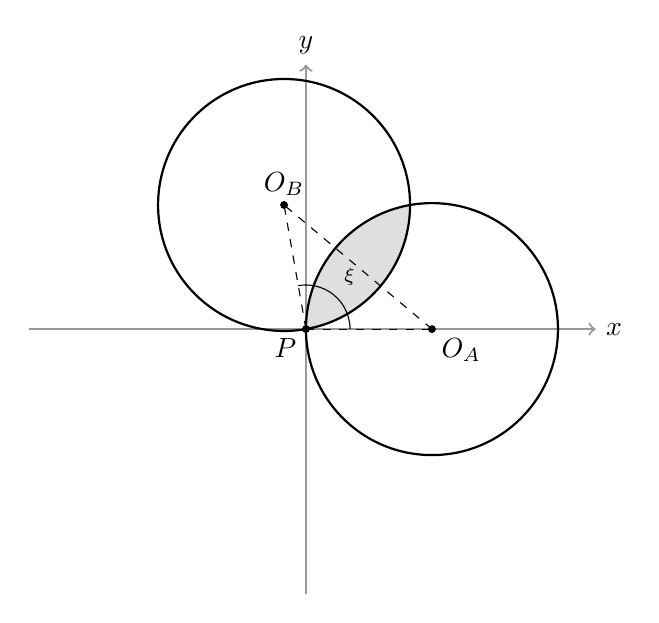
\begin{tikzpicture}[scale=1.6]

  % --- 3. 座標軸 ---
  \draw[->, thick, gray!80] (-2.2, 0) -- (2.3, 0) node[right, black] {$x$};
  \draw[->, thick, gray!80] (0, -2.1) -- (0, 2.1) node[above, black] {$y$};

  % 中心角theta=100度の例で図示 (0<=theta<=pi の範囲内)
  \coordinate (P) at (0,0);
  \coordinate (OA) at (1,0);
  \coordinate (OB) at ({cos(100)},{sin(100)});
  % 2円板の共通部分 (斜線部) の面積がS(theta)
  \fill[gray!25] (P) arc (180:100:1) arc (0:-80:1);
  \draw[thick] (OA) circle (1);
  \draw[thick] (OB) circle (1);
  \draw[dashed] (P) -- (OA);
  \draw[dashed] (P) -- (OB);
  \draw[dashed] (OA) -- (OB);
  \draw (0.35,0) arc (0:100:0.35) node[midway,above right]{\scriptsize$\xi$};
  \filldraw (P) circle(0.75pt) node[below left]{$P$};
  \filldraw (OA) circle(0.75pt) node[below right]{$O_A$};
  \filldraw (OB) circle(0.75pt) node[above]{$O_B$};
\end{tikzpicture}
\caption{中心角$\xi$の2円板の共通部分（斜線部）の面積が$S(\xi)$}
\end{figure}

\begin{figure}[htb]
\begin{center}
\begin{tikzpicture}[scale=2.6, >=stealth]

  % --- 1. パラメータ設定 (例: xi = 70度) ---
  \def\xiVal{70}
  \pgfmathsetmacro{\sinHalf}{sin(\xiVal/2)}       % sin(xi/2) ≒ 0.5736
  \pgfmathsetmacro{\distTwo}{2*\sinHalf}          % 中心間距離 2*sin(xi/2) ≒ 1.1472
  \pgfmathsetmacro{\yIntersect}{sqrt(1 - \sinHalf*\sinHalf)} % 交点の y 座標 = cos(xi/2)

  \coordinate (O1) at (0, 0);
  \coordinate (O2) at (\distTwo, 0);

  % --- 2. 共通部分のハッチング ---
  % 全体の共通部分
  \begin{scope}
    \clip (O1) circle (1.0);
    \clip (O2) circle (1.0);
    \fill[blue!10] (-0.2, -1.1) rectangle (1.8, 1.1);
    
    % 第1象限の積分対象部分 (4倍する基本領域) を濃い斜線で強調
    \fill[pattern=north east lines, pattern color=blue!80!black] 
      (\sinHalf, 0) -- plot[domain=\sinHalf:1.0, samples=40] (\x, {sqrt(1 - \x*\x)}) 
      -- (1.0, 0) -- cycle;
  \end{scope}

  % --- 3. 座標軸 ---
  \draw[->, thick] (-1.3, 0) -- (2.4, 0) node[right] {$x$};
  \draw[->, thick] (0, -1.3) -- (0, 1.4) node[above] {$y$};
  \node[below left, font=\small] at (0,0) {$O$};

  % --- 4. 2つの円の描画 ---
  % 円 1: x^2 + y^2 = 1
  \draw[ultra thick, blue!80!black] (O1) circle (1.0);
  \node[blue!80!black, font=\small, above left] at (-0.6, 0.7) {$x^2+y^2=1$};

  % 円 2: (x - 2sin(xi/2))^2 + y^2 = 1
  \draw[ultra thick, red!80!black] (O2) circle (1.0);

  % --- 5. 交線 x = sin(xi/2) (破線) ---
  \draw[thick, dashed, purple!80!black] (\sinHalf, -\yIntersect - 0.2) -- (\sinHalf, \yIntersect + 0.3)
    node[above, font=\small] {$x = \sin\dfrac{\xi}{2}$};

  % --- 6. 目盛りとラベル ---
  % 交点の x 座標
  \fill[purple!80!black] (\sinHalf, 0) circle (1.0pt) 
    node[below left, font=\small] {$\sin\dfrac{\xi}{2}$};

  % 円 1 の端点 x = 1
  \fill[black] (1.0, 0) circle (1.0pt) node[below right, font=\small] {$1$};

  % 円 2 の中心 (2sin(xi/2), 0)
  \fill[red!80!black] (O2) circle (1.2pt) 
    node[below right, font=\small] {$2\sin\dfrac{\xi}{2}$};

  % 曲線 y = sqrt(1-x^2) の注記
  \draw[->, thin, blue!80!black] (0.85, 0.75) to[bend right=15] (0.8, {sqrt(1 - 0.8*0.8)});
  \node[blue!80!black, font=\scriptsize, above right] at (0.85, 0.75) {$y = \sqrt{1-x^2}$};

  % 基本面積（第1象限の1/4）のラベル
  \node[blue!90!black, font=\scriptsize] at (0.72, 0.22) {$\displaystyle\int_{\sin\frac{\xi}{2}}^1 \sqrt{1-x^2}\,dx$};

  % 全体面積 S(xi) の注記
  \node[black, font=\small] at (0.6, -0.6) {$S(\xi) = 4 \times (\text{斜線部})$};

\end{tikzpicture}
\end{center}
\caption{中心間距離 $2\sin\dfrac{\xi}{2}$ に配置した 2 円の共通部分 $S(\xi)$ と積分区間}
\end{figure}

さて，中心間の偏角の差が$\xi$（$0\le\xi\le\pi$）である2つの単位円板の共通部分の面積を$S(\xi)$とする．
2円の中心間距離は$2\sin\dfrac{\xi}{2}$なので図よりこの面積は
\begin{align}
 S(\xi)
  &=4\int_{\sin\frac{\xi}{2}}^1\sqrt{1-x^2}\,dx \\
  &=4\int_{\frac{\xi}{2}}^{\frac{\pi}{2}}\cos^2t\,dt \quad (x = \sin t)\\
  &=4\Bigl[\dfrac{t}{2}+\dfrac{\sin2t}{4}\Bigr]_{\frac{\xi}{2}}^{\frac{\pi}{2}} \\
  &=\pi-\xi-\sin\xi \label{eq:5}
\end{align}
である．

$O_A,O_B,O_C$の偏角はそれぞれ$0,\theta,\alpha$（$0\le\theta\le\pi\le\alpha\le\theta+\pi$）なので，これらを結ぶ3つの弧の中心角は
\begin{align}
\overset{\frown}{O_AO_B}=\theta,\qquad\overset{\frown}{O_BO_C}=\alpha-\theta,\qquad\overset{\frown}{O_CO_A}=2\pi-\alpha
\end{align}
である．
3円板の和集合の面積$S$は，3円の面積の和から2円ずつの重なりを引けば得られるから
\begin{align}
 S=3\pi-\bigl\{S(\theta)+S(\alpha-\theta)+S(2\pi-\alpha)\bigr\}
\end{align}
と書ける．\cref{eq:5}を代入して
\begin{align}
 S
  &= 3\pi - 3\pi + \left(\theta+(\alpha-\theta) + (2\pi-\alpha)\right) + \sin\theta + \sin(\alpha-\theta) + \sin(2\pi-\alpha) \\
  &= 2\pi + \sin\theta + \sin(\alpha-\theta) + \sin(-\alpha) \label{eq:6}
\end{align}
である．
和積公式から
\begin{align}
 \sin(\alpha-\theta)+\sin(-\alpha)=-2\sin\dfrac{\theta}{2}\cos\Bigl(\alpha-\dfrac{\theta}{2}\Bigr)
\end{align}
だから代入して
\begin{align}
 S &= 2\pi-2\sin\dfrac{\theta}{2}\cos\Bigl(\alpha-\dfrac{\theta}{2}\Bigr)+\sin\theta \label{eq:7}
\end{align}
を得る．
\cref{eq:2,eq:4}の元でこの最大値を求めれば良い．
まず$\theta$を固定して$\alpha$を動かす．
\cref{eq:2,eq:4}より
\begin{align}
 \begin{cases}
   \pi-\dfrac{\theta}{2} \le \alpha-\dfrac{\theta}{2} \le \pi+\dfrac{\theta}{2} \\
   0\le\theta\le\pi
 \end{cases}
\end{align}
である．

\begin{figure}[htb]
\begin{center}
\begin{tikzpicture}[scale=1.5, >=stealth]

  % --- 1. 定数・スケール設定 ---
  % pi ≒ 3.1416 を描画用にスケーリング
  \def\piVal{3.14159}

  % 頂点座標の定義: (theta, Y = alpha - theta/2)
  % theta = 0 のとき: Y = pi
  % theta = pi のとき: Y は pi/2 から 3pi/2
  \coordinate (O) at (0, 0);
  \coordinate (P_left) at (0, \piVal);
  \coordinate (P_top)  at (\piVal, {1.5*\piVal});
  \coordinate (P_bot)  at (\piVal, {0.5*\piVal});

  % --- 2. 存在領域の斜線ハッチング ---
  \fill[pattern=north east lines, pattern color=blue!70] 
    (P_left) -- (P_top) -- (P_bot) -- cycle;

  % --- 3. 座標軸 ---
  \draw[->, thick] (-0.3, 0) -- ({\piVal + 0.8}, 0) node[right] {$\theta$};
  \draw[->, thick] (0, -0.3) -- (0, {1.5*\piVal + 0.8}) node[above] {$\alpha - \dfrac{\theta}{2}$};
  \node[below left, font=\small] at (0,0) {$O$};

  % --- 4. 領域の境界線の描画 ---
  % 上辺: Y = pi + theta/2
  \draw[thick, blue!80!black] (P_left) -- (P_top) 
    node[midway, above left, font=\scriptsize, rotate=17] {$\alpha - \dfrac{\theta}{2} = \pi + \dfrac{\theta}{2}$};

  % 下辺: Y = pi - theta/2
  \draw[thick, blue!80!black] (P_left) -- (P_bot) 
    node[midway, below left, font=\scriptsize, rotate=-17] {$\alpha - \dfrac{\theta}{2} = \pi - \dfrac{\theta}{2}$};

  % 右辺 (theta = pi の境界)
  \draw[thick, blue!80!black] (P_bot) -- (P_top);

  % --- 5. 最大値を与える中心線 (Y = pi) ---
  \draw[ultra thick, red!80!black, dashed] (0, \piVal) -- ({\piVal + 0.3}, \piVal)
    node[right, font=\small] {$\alpha - \dfrac{\theta}{2} = \pi$（$S$ が最大）};

  % 最大点 theta = 2pi/3 のプロット
  %\coordinate (MaxPt) at ({2*\piVal/3}, \piVal);
  %\draw[dashed, gray] ({2*\piVal/3}, 0) node[below, black, font=\small] {$\dfrac{2\pi}{3}$} -- (MaxPt);
  %\fill[red!80!black] (MaxPt) circle (2.0pt) 
  %  node[above right, font=\scriptsize] {最大点};

  % --- 6. 目盛りとラベル ---
  % 縦軸の目盛り
  \draw[dashed, gray] (P_top) -- (0, {1.5*\piVal}) node[left, font=\small] {$\dfrac{3\pi}{2}$};
  \draw[dashed, gray] (P_bot) -- (0, {0.5*\piVal}) node[left, font=\small] {$\dfrac{\pi}{2}$};
  \node[left, font=\small] at (0, \piVal) {$\pi$};

  % 横軸の目盛り
  \draw[dashed, gray] (\piVal, 0) node[below, font=\small] {$\pi$} -- (P_bot);

  % 領域ラベル
  \node[blue!90!black, font=\large] at ({0.6*\piVal}, \piVal) {$D$};

\end{tikzpicture}
\end{center}
\caption{$(\theta, \alpha - \theta/2)$ の存在領域（斜線部）}
\end{figure}

$\sin\dfrac{\theta}{2} \ge 0$および上図から，$\alpha-\dfrac{\theta}{2} = \pi$の時に$S$は最大となり
\begin{align}
  \max S &=2\sin\dfrac{\theta}{2}+\sin\theta\equiv g(\theta)\qquad(0\le\theta\le\pi)
\end{align}
をとる．これを$f(\theta)$とおいて，次に$\theta$を動かす．
一階微分は
 \begin{align}
  f'(\theta) 
   &= \cos\dfrac{\theta}{2} + \cos\theta \\
   &= \cos\dfrac{\theta}{2} + 2\cos^2\dfrac{\theta}{2} -1 \\
   &= \left(2\cos\dfrac{\theta}{2} - 1\right)\left(\cos\dfrac{\theta}{2} + 1\right)
 \end{align}
だから$f(\theta)$の増減表は以下のようになる．

従って$f(\theta)$は$\theta = \dfrac{2\pi}{3}$で最大値をとり，その値は
\begin{align}
 \max S 
  &= f\left(\dfrac{2\pi}{3}\right) \\
  &= 2\pi + \dfrac{3\sqrt{3}}{2} 
\end{align}
である．


{\bf [解説]}

$S$が最大値の時，$\theta=\dfrac{2\pi}{3}$，$\alpha=\pi+\dfrac{\theta}{2}=\dfrac{4\pi}{3}$となるから，3つの弧の中心角は
\begin{align}
\overset{\frown}{O_AO_B}=\overset{\frown}{O_BO_C}=\overset{\frown}{O_CO_A}=\dfrac{2\pi}{3}
\end{align}
となり，3つの中心が$P$のまわりに正三角形状に等間隔配置されるときに最大値が実現される．

\begin{figure}[htb]
\centering
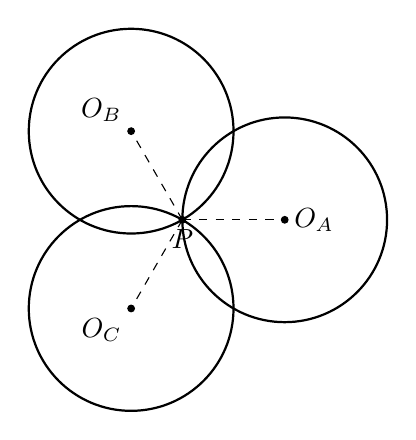
\begin{tikzpicture}[scale=1.3]
  % theta=alpha-theta=2pi-alpha=2pi/3 の等間隔配置 (Sが最大となる配置)
  \foreach \a in {0,120,240}{
    \coordinate (O\a) at ({cos(\a)},{sin(\a)});
    \draw[thick] (O\a) circle (1);
    \filldraw (O\a) circle(0.92pt);
    \draw[dashed] (0,0) -- (O\a);
  }
  \filldraw (0,0) circle(0.92pt) node[below]{$P$};
  \node[right] at (O0) {$O_A$};
  \node[above left] at (O120) {$O_B$};
  \node[below left] at (O240) {$O_C$};
\end{tikzpicture}
\caption{$S$が最大となる配置（3つの中心が$P$のまわりに等間隔）}
\end{figure}


\newpage

\end{document}
